\begin{mainquestion}{bridgefilter}{Bridge Circuit Analysis}

\questionpoints
Consider the bridge circuit shown below.

\begin{center}
\begin{circuitikz}[american voltages]
    % Source branch (stretched height to 6)
    \draw (0,0) to[sV, l=$V_{in}$] (0,6);

    % Top and Bottom Rails (stretched width to 8)
    \draw (0,6) -- (8,6);
    \draw (0,0) -- (8,0);

    % Middle Branch (moved from x=2 to x=4)
    \draw (4,6) to[R, l=$1~k\Omega$] (4,3) 
                to[R, l=$2~k\Omega$] (4,0);

    % Right Branch (moved from x=4 to x=8)
    \draw (8,6) to[R, l=$2~k\Omega$] (8,3) 
                to[R, l=$1~k\Omega$] (8,0);

    % Capacitor Bridge (connecting the wider gap)
    \draw (4,3) to[C, l={$C=10~\mu F$}, v={$V_{out}$}] (8,3);

    % Connection Nodes
    \draw (4,3) node[circ]{};
    \draw (8,3) node[circ]{};
\end{circuitikz}
\end{center}

% =========================================================
\begin{partquestion}{transferfunction}
{Find the transfer function $H(\omega) = \frac{V_{out}}{V_{in}}$. \\
    \textbf{Hint:} Find a Thévenin equivalent circuit for the bridge as seen by the capacitor terminals first.}

\begin{answer}[3in]
        To find the Thévenin equivalent seen by the capacitor, we remove the capacitor and find the open-circuit voltage ($V_{Th}$) and the equivalent resistance ($R_{Th}$) looking into the terminals.

        \textbf{1. Find $V_{Th}$ (Open Circuit Voltage):}
        The circuit becomes two parallel voltage dividers.
        \[V_{left} = V_{in} \left( \frac{2k\Omega}{1k\Omega + 2k\Omega} \right) = V_{in} \left( \frac{2}{3} \right)\]
        \[V_{right} = V_{in} \left( \frac{1k\Omega}{2k\Omega + 1k\Omega} \right) = V_{in} \left( \frac{1}{3} \right)\]
        
        The schematic defines $V_{out}$ from left to right ($V_{left} - V_{right}$).
        \[V_{Th} = V_{left} - V_{right} = \frac{2}{3}V_{in} - \frac{1}{3}V_{in} = +\frac{1}{3}V_{in}\]

        \textbf{2. Find $R_{Th}$ (Thévenin Resistance):}
        We turn off the source $V_{in}$ (short circuit). The resistors in each branch become parallel combinations connected in series.
        \[R_{left} = 1k\Omega \parallel 2k\Omega = \frac{1 \cdot 2}{1 + 2} k\Omega = \frac{2}{3} k\Omega\]
        \[R_{right} = 2k\Omega \parallel 1k\Omega = \frac{2 \cdot 1}{2 + 1} k\Omega = \frac{2}{3} k\Omega\]
        \[R_{Th} = R_{left} + R_{right} = \frac{2}{3} k\Omega + \frac{2}{3} k\Omega = \frac{4}{3} k\Omega \approx 1333~\Omega\]

        \textbf{3. Build Transfer Function:}
        The equivalent circuit is $V_{Th}$ in series with $R_{Th}$ and the capacitor $C$. We use a voltage divider:
        \[V_{out} = V_{Th} \cdot \frac{Z_C}{R_{Th} + Z_C} = \left(\frac{1}{3}V_{in}\right) \frac{\frac{1}{j\omega C}}{R_{Th} + \frac{1}{j\omega C}}\]
        Multiply numerator and denominator by $j\omega C$:
        \[H(\omega) = \frac{V_{out}}{V_{in}} = \frac{1}{3} \cdot \frac{1}{1 + j\omega R_{Th} C}\]
        
        Substituting values ($R_{Th} = 1333~\Omega$, $C = 10~\mu F$):
        \[R_{Th}C = 1333 \cdot 10 \cdot 10^{-6} \approx 0.0133\]
        \[H(\omega) = \frac{1/3}{1 + j\omega(0.0133)}\]
\end{answer}

\end{partquestion}

% =========================================================
\begin{partquestion}{functionality}
{Based on the result from (a), identify the functionality of this circuit (what does it do?).}

\begin{answer}[0.5in]
        The transfer function is of the form $\frac{K}{1 + j(\omega/\omega_c)}$. This represents a **Low Pass Filter**. The gain is positive ($+1/3$), indicating it is non-inverting.
\end{answer}

\end{partquestion}

% =========================================================
\begin{partquestion}{bodesketch}
{Plot a sketch (to scale) of $|H(\omega)|$ and $\angle H(\omega)$.}

\begin{answer}[4.5in]
        The magnitude is $|H(\omega)| = \frac{1/3}{\sqrt{1 + (\omega R_{Th} C)^2}}$.
        The phase is $\angle H(\omega) = -\arctan(\omega R_{Th} C)$.
        
        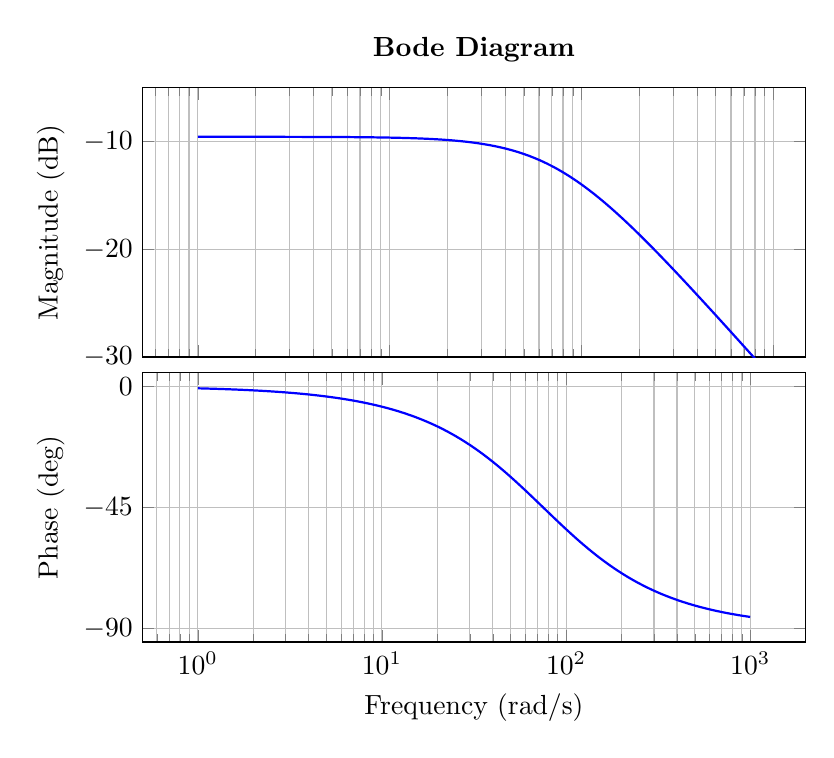
\begin{tikzpicture}
            % Magnitude Plot
            \begin{axis}[
                name=magplot,
                width=10cm, height=5cm,
                xmode=log,
                title=\textbf{Bode Diagram},
                ylabel={Magnitude (dB)},
                ymin=-30, ymax=-5,
                grid=both,
                xticklabels=\empty
            ]
            % 20*log10(1/3) is approx -9.54 dB
            \addplot[blue, thick, domain=1:1000, samples=100] {20*log10( (1/3) / sqrt(1 + (x/75)^2) )};
            \end{axis}
            
            % Phase Plot - Stacked below
            \begin{axis}[
                name=phaseplot,
                at={(magplot.south west)}, anchor=north west, yshift=-0.2cm,
                width=10cm, height=5cm,
                xmode=log,
                ylabel={Phase (deg)},
                xlabel={Frequency (rad/s)},
                ymin=-95, ymax=5,
                ytick={0, -45, -90},
                grid=both
            ]
            \addplot[blue, thick, domain=1:1000, samples=100] {-atan(x/75)};
            \end{axis}
        \end{tikzpicture}
\end{answer}

\end{partquestion}

% =========================================================
\begin{partquestion}{cornerfrequency}
{What is the corner frequency $\omega_c$?}

\begin{answer}[1in]
        The corner frequency occurs when the real and imaginary parts of the denominator are equal ($ \omega R_{Th} C = 1 $).
        \[\omega_c = \frac{1}{R_{Th}C} = \frac{1}{(4000/3~\Omega) (10 \cdot 10^{-6}~F)}\]
        \[\omega_c = \frac{3}{40 \cdot 10^{-3}} = \frac{3000}{40} = 75 \text{ rad/s}\]
\end{answer}

\end{partquestion}

% =========================================================
\begin{partquestion}{outputvoltage}
{What is the output voltage if the input voltage is $v_{in}(t) = 5 + 3\cos(50t) + 2\sin(200t)$ V?}

\begin{answer}[2in]
        We apply superposition for each frequency component:
        
        1. **DC Component ($V_{in} = 5$):** $\omega = 0$.
        \[H(0) = 1/3\]
        \[V_{out,0} = 5 \cdot (1/3) = 1.67~\text{V}\]

        2. **$\omega = 50$ rad/s:**
        \[H(j50) = \frac{1/3}{1 + j(50/75)} = \frac{0.333}{1 + j0.667}\]
        \[|H| = \frac{0.333}{\sqrt{1 + 0.667^2}} \approx 0.277\]
        \[\angle H = -\arctan(0.667) = -33.7^\circ\]
        \[v_{out,1}(t) = 3(0.277)\cos(50t - 33.7^\circ) = 0.83\cos(50t - 33.7^\circ)\]

        3. **$\omega = 200$ rad/s:**
        \[H(j200) = \frac{1/3}{1 + j(200/75)} = \frac{0.333}{1 + j2.667}\]
        \[|H| = \frac{0.333}{\sqrt{1 + 2.667^2}} \approx 0.117\]
        \[\angle H = -\arctan(2.667) = -69.4^\circ\]
        \[v_{out,2}(t) = 2(0.117)\sin(200t - 69.4^\circ) = 0.234\sin(200t - 69.4^\circ)\]

        **Total Output:**
        \[v_{out}(t) = 1.67 + 0.83\cos(50t - 33.7^\circ) + 0.23\sin(200t - 69.4^\circ) \text{ V}\]
\end{answer}

\end{partquestion}

\end{mainquestion}
